\Chapter{Introduction}
	\section{Fondamentaux de la physique des plasmas}
		\emph{La vie non examinée n'est pas digne d'être vécue }- Socrate. 
		
		Dans la recherche de la connaissance et de la compréhension ce monde qui
		l'entoure, l'homme s'est tout d'abord intéressé à la matière qui le compose. Celle-ci
		peut nous apparaître sous trois états principaux : lorsque les atomes,
		structures élementaires de la matière, sont immobiles \emph{ie.} à très faible
		température, on parle d'état solide de la matière. En les laissant se déplacer
		les uns par rapport aux autres, la matière devient déformable et prend alors
		la forme d'un liquide. Enfin, une élévation de l'énergie des particules leur
		permettant une plus grande liberté, la matière se trouve à l'état gazeux, 
		tendant à occuper tout l'espace qui se trouve à sa disposition.
		
		Il existe cependant un état plus exotique de la matière, \emph{le plasma}. Cet
		état réprésente plus de 99\% de la matière connue mais nous n'avons pris conscience
		de son existence que très tardivement. Il apparaît en effet dans des
		conditions de température et de pression très différentes de celles de notre
		atmosphère terrestre. A très haute température, la dissociation des
		molécules puis l'ionisation des atomes donne naissance à une
		population d'ions et d'électrons libres. Celle-ci va fortement influencer le
		comportement global du gaz, en le rendrant sensible aux champs
		électromagnétiques, et provoquant de plus des phénomènes collectifs,
		non-linéaires et turbulents. Le plasma et son comportement sont décris par la
		théorie de la physique des plasmas. Elle intègre les connaissances de
		nombreux domaines, tels que la physique statistique, l'électromagnétisme, ou
		encore la dynamique des fluides. 
		
		\subsection{Zoologie des plasmas}
			Les plasmas se divisent essentiellement en trois catégories : les plasmas
			naturels, les plasmas industriels et les plasmas thermonucléaires.
			\begin{figure}
				\centering
				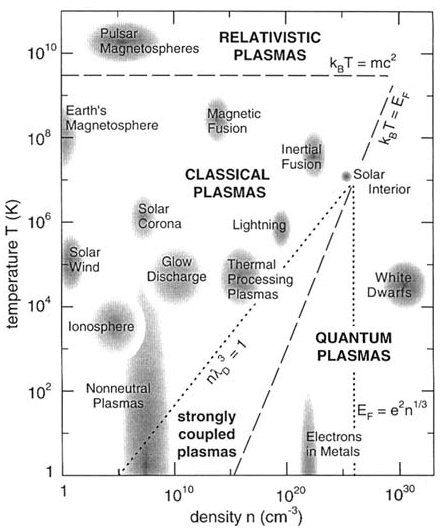
\includegraphics[height=100mm,width=80mm]{figures/zoologie.png}{\caption{Classification
				de différents plasmas en fonction de $n_e$ et $T_e$.}\label{zoologie}}
			\end{figure}
			La figure \ref{zoologie} issue de \cite{national1995Plasma} représente une
			classification des plasmas en fonction de leur deux principales
			caractéristiques : 
			\begin{itemize}
				\item la densité électronique $n_e$ détermine le degré d'ionisation du plasma :
				$$\alpha=\frac{n_e}{n_e+n_i}$$ 
				\item la température électronique $T_e$ définit
			l'agitation thermique et contrôle la cinétique du plasma à travers le paramètre plasma\footnote{Le paramètre 
			plasma représente le ratio
			entre l'énergie thermique des électrons et leur énergie potentielle electrostatique coulombienne 
			\emph{ie.} l'inertie des électrons (et principalement leur agitation thermique desordonnée) contre les forces
			d'interactions coulombiennes structurantes. La tendance au chaos, ou à l'ordonnancement.}
			$$\Gamma=\frac{<E_p>}{<E_c>}=\frac{e^2n_e^{1/3}}{\epsilon_0 kT_e}$$
			\end{itemize}
			
			Le dégré d'ionisation va fortement influencer la nature du transport des courants dans le plasma.
			le paramètre des charges et 
			  
			ont une vitesse supérieure à $c$ la vitesse de la lumière, les effets
			relativistes sont importants. A forte densité, 
			
			\lipsum{50}
		\subsection{Plasma parameters}
		 Plasma parameter $\Lambda$ Debye sphere, Quasineutrality Debye length,
		Electrostatic plasma frequency $\omega_c$
		 Density : Degree of ionisation $\alpha=n_i/(n_i+n_n)$
			Temperature : Saha equation, thermal equilibrium, Maxwellian energy dist function
			Potentials : Debye sheath, Boltzmann relation
			Magnetization : Hall parameter, Larmor radius, plasma frequency
			\lipsum{50}
		\subsection{Collective behaviour}
			Ambipolar field, heating, drifts
		\subsection{Collisions}
			\lipsum{50}
		\subsection{Scales}
			\lipsum{50}
		
	\section{Fluid description of a plasma}
	\lipsum{50}
		\subsection{Statistical description}
			\subsubsection{BBGKY hierarchy, liouville equation}
			\subsubsection{The Boltzmann equation}
			\lipsum{50}
		\subsection{Moments of the Boltzmann equation, conservation laws}
			Braginskii equations
			\subsubsection{Continuity equation}
			\lipsum{50}
			\subsubsection{Momentum equation}
			\lipsum{50}
			\subsubsection{Energy equation}
			\lipsum{50}
			\subsubsection{Heat equation}
			\lipsum{50}
	\section{Low-temperature plasmas}
		\subsection{Creation of the discharge, role of electrons}
		Dans les plasmas basse-température industriels et de laboratoires, qui possédent
			un faible degré d'ionisation, ou dans l'ionospère, la dynamique du plasma est dominée par
			la perte de quantité de mouvement dûe à l'ionisation la force de friction avec le gaz.
		Electrical breakdown, Townsend avalanche, 
		\lipsum{50}
		\subsection{Ions transport and ambipolar field}
	\section{Edge plasma physics of tokamaks}
		Lawson criteriom, strongly magnetized
		\subsection{Fusion and tokamaks}
		\subsection{Drift velocities}
		\subsection{Turbulence and anomalous transverse transport}
		\lipsum{50}
	\section{Plasma surface interaction and sheath physics}
		\lipsum{50}
		\subsection{Debye sheath}
			\lipsum{50}
		\subsection{Bohm criterium}
			\lipsum{50}
		\subsection{Open field line physics}
			\lipsum{50}
		\subsection{Issue of sheath parallel to the magnetic field}
			\lipsum{50}

		